\EN{The Hirota--Satsuma coupled KdV (HScKdV) system [1, 2],}
\CN{Hirota--Satsuma 耦合 KdV（HScKdV）系统 [1,2] 为}
\begin{equation}
\originaleq{1.1}
\begin{cases}
u_t=\dfrac{1}{2}u_{xxx}-3uu_x+6vv_x,\\
v_t=-v_{xxx}+3uv_x,
\end{cases}
\end{equation}
\EN{can be used to describe the interaction of two long waves with different dispersion relations, which is reduced to the KdV equation [3, 4] when $v=0$.}
\CN{它可描述具有不同色散关系的两种长波之间的相互作用；当 $v=0$ 时，系统约化为 KdV 方程 [3,4]。}
\begin{proof}
\textbf{约化的补充验证。}
代入 $v\equiv0$ 后，第二式两边恒为零，第一式为 $u_t=\dfrac{1}{2}u_{xxx}-3uu_x$。
若希望与常用形式对照，令 $q(x,\tau)=-u(x,-2\tau)$，链式法则给
\[
q_\tau=2u_t=u_{xxx}-6uu_x=-q_{xxx}-6qq_x,
\]
即 $q_\tau+6qq_x+q_{xxx}=0$。
这里的变量变换用于比较不同文献的 KdV 系数约定，不是证明中为缩短公式所设的简记。
\end{proof}
\begin{note}
物理解释中的“色散关系”可从零解附近的线性化理解。
忽略二次项，分别代入平面波 $e^{\ii(\xi x-\omega t)}$，有
$-\ii\omega=-\dfrac{\ii\xi^3}{2}$ 与 $-\ii\omega=\ii\xi^3$，
因此两分量的线性色散关系分别为 $\omega=\dfrac{1}{2}\xi^3$ 和 $\omega=-\xi^3$。
二次项描述分量之间及同一分量内部的非线性耦合；这项线性化计算说明“不同色散”的数学含义，不替代物理模型的推导。
\end{note}
\EN{System (1.1) has been studied extensively since it was proposed.}
\CN{系统 (1.1) 自提出以来已得到广泛研究。}
\EN{Soliton solutions of the HScKdV system are obtained by using the bilinear method [1].}
\CN{文献 [1] 用双线性方法求得了 HScKdV 系统的孤子解。}
\EN{It is also showed that the HScKdV system is a four-reduction of the well-known Kadomtsev--Petviashvili hierarchy [2].}
\CN{文献 [2] 还表明该系统是著名的 Kadomtsev--Petviashvili（KP）层级的四约化。}
\EN{Dodd showed this system is completely integrable in the sense of having a Lax pair [5].}
\CN{Dodd 从存在 Lax 对的意义说明了该系统的完全可积性 [5]。}
\EN{More exact solutions under nonzero background are obtained by Tam et al. [6].}
\CN{Tam 等人在非零背景下求得了更多精确解 [6]。}
\EN{Levi constructed the B\"acklund transformation for this system [7].}
\CN{Levi 构造了该系统的 B\"acklund 变换 [7]。}
\EN{Hu and Liu gave its binary Darboux transformation [8].}
\CN{Hu 与 Liu 给出了该系统的二元 Darboux 变换 [8]。}
\EN{A three-component generalization of this system is given in Ref. [9].}
\CN{文献 [9] 给出了该系统的三分量推广。}
\EN{To the best of our knowledge, no one has performed inverse scattering analysis on this system so far.}
\CN{据作者所知，截至该文写作时尚无人对这一系统开展逆散射分析。}
\EN{The aim of this work is to fill this gap.}
\CN{本文旨在填补这一空白。}
\begin{note}
以上是原文的文献史陈述，参考文献序号按原文保留；“据作者所知”的时间范围是原论文写作时，不能读成持续到现在的检索结论。
双线性方法将方程改写成适于构造行波与多孤子的双线性算子方程；B\"acklund、Darboux 变换用于从已知解生成新解。
KP 层级的四约化是对层级中的算子施加四阶约化约束，不是简单令第四个时间变量为零。
这些历史结果不是后文证明所依赖的额外假设；本文实际使用的 Lax 对会在第 2.1 节逐项独立验证。
\end{note}

\begin{figure}[htbp]
\centering
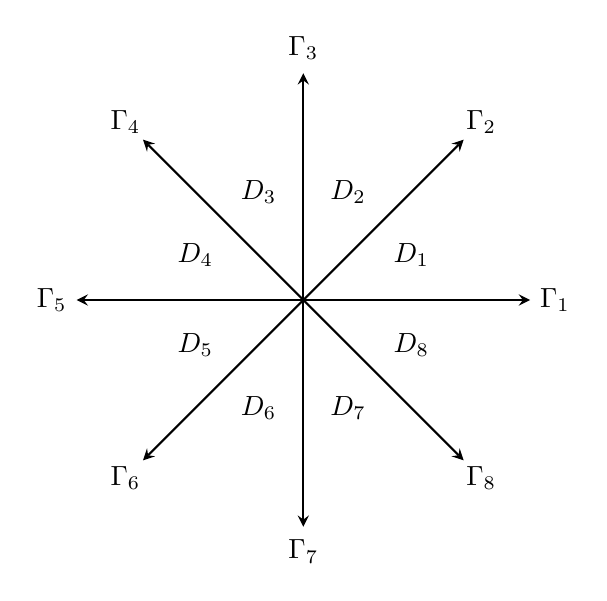
\begin{tikzpicture}[scale=0.9,>=stealth]
\foreach \j in {1,...,8}{
 \pgfmathsetmacro{\ang}{45*(\j-1)}
 \draw[->,thick] (0,0)--(\ang:3.2);
 \node at (\ang:3.55) {$\Gamma_{\j}$};
 \pgfmathsetmacro{\midang}{\ang+22.5}
 \node at (\midang:1.65) {$D_{\j}$};
}
\end{tikzpicture}
\refstepcounter{figure}
\caption*{\textbf{Figure 1／图 1.} The contour $\Gamma=\displaystyle\bigcup\limits_{j=1}^8\Gamma_j$ and the open sets $\{D_j\}_{j=1}^8$.\par
轮廓 $\Gamma$ 与八个开区域；所有射线均从原点指向无穷远。按原图重新绘制。}
\label{fig:sectors}
\end{figure}

\EN{Solving integrable nonlinear partial differential equations by the inverse scattering transform (IST) is an important milestone in soliton theory.}
\CN{用逆散射变换（inverse scattering transform，IST）求解可积非线性 PDE，是孤子理论的重要里程碑。}
\EN{The modern version of the IST method usually relies on dealing with the associated Riemann--Hilbert (RH) problem [10], so it is also called the RH method.}
\CN{现代 IST 通常依赖相应的 RH 问题 [10]，因此也称为 RH 方法。}
\EN{The advantage of this method is that once the relevant RH problem is established, not only the soliton solution can be obtained in reflectionless case, but also the Deift--Zhou steepest descent method [11] can be applied to study the asymptotic behavior of the solutions [12--14].}
\CN{其优点在于：建立 RH 问题后，既可在无反射情形求孤子解，也可用 Deift--Zhou 最速下降方法 [11] 研究解的渐近行为 [12--14]。}
\EN{This is one of our main motivations for deriving RH representations for solutions of the HScKdV system.}
\CN{这也是作者为 HScKdV 系统建立 RH 表示的主要动机之一。}
\EN{We hope to analyze the long-time asymptotic behavior of the solution for the HScKdV system in the following work.}
\CN{作者希望在后续工作中分析该系统解的长时间渐近行为。}
\begin{note}
这里的两个用途共享同一个谱表示，但求解技术不同。
无反射时跳跃可化为单位矩阵，逆问题由极点条件与归一化决定，可归结为有限维线性代数。
有反射时跳跃带振荡指数，长时间分析需要对 RH 问题变形、局部模型和误差估计。
后一个计划在本论文中尚未完成，故本笔记不把它写成本文定理。
\end{note}

\EN{The main difficulties we encountered in this paper are as follows.}
\CN{本文遇到的主要困难如下。}
\EN{It is well-known that in the inverse scattering analysis, in order to correctly recover the solutions of the associated soliton equation, it is necessary to fully characterize the symmetries of the eigenfunctions and the scattering data.}
\CN{逆散射分析中，为正确恢复相应孤子方程的解，需要充分刻画特征函数和散射数据的对称性。}
\EN{Therefore, the corresponding Lax pair is required to have a ``good'' symmetry.}
\CN{因此，相应 Lax 对应具有适合分析的对称性。}
\EN{We first observe that the Lax pair of system (1.1) (see (2.1)) is very irregular and not suitable for inverse scattering analysis.}
\CN{作者首先观察到，系统 (1.1) 的 Lax 对（见 (2.1)）形式不规则，不适于直接开展逆散射分析。}
\EN{Therefore, we need to find a gauge transformation (see (2.3)) that converts the Lax pair to the Zakharov--Shabat-type spectral problems.}
\CN{因此，需要寻找规范变换（见 (2.3)），将 Lax 对变为 Zakharov--Shabat 型谱问题。}
\EN{Since the transformed Lax pair has a more complex form, it is very difficult to find a suitable symmetry.}
\CN{变换后的 Lax 对形式较复杂，寻找合适对称性仍然困难。}
\EN{But fortunately, after a detailed calculation, we finally found three suitable symmetries, which allowed our inverse scattering analysis to proceed smoothly.}
\CN{经过细致计算，作者最终找到三种合适的对称关系，使逆散射分析能够进行。}
\begin{note}
“适合分析”是关于表示形式的评价，不是额外的数学假设。
背景对角化后，相位由对角特征值明确给出，逐列解析域才能通过指数的实部排序读出。
第 2.1 节先证明谱旋转与复共轭关系；后文还需伴随及相应矩阵关系来完成实值重构。
不能从这里的“三种”反推引理 2.1 本身已经列出三种独立变换。
\end{note}
\EN{Note that the Lax pair of the HScKdV system is fourth order, which makes the inverse scattering analysis extremely difficult.}
\CN{注意，该系统的 Lax 对为四阶，这使逆散射分析显著复杂。}
\EN{In the low-order case (such as the nonlinear Schr\"odinger [NLS] equation), we need to define the fundamental matrix meromorphic eigenfunctions of the corresponding Lax pair in the upper half complex plane and the lower half complex plane, and use them to derive the related RH problem.}
\CN{低阶情形（例如 NLS 方程）中，通常在上、下半平面定义相应 Lax 对的基本亚纯矩阵特征函数，再由它们建立 RH 问题。}
\EN{Such fundamental matrix eigenfunction solution is called the Beals--Coifman simultaneous solution of the corresponding Lax pair [15].}
\CN{这种基本矩阵特征函数解称为相应 Lax 对的 Beals--Coifman 共同解 [15]。}
\EN{One usually use the Jost solutions of the Lax pair to define the Beals--Coifman simultaneous solution, because there are two columns of analytic Jost solutions in each half-plane.}
\CN{通常可以用 Jost 解拼出 Beals--Coifman 共同解，因为每个半平面中有两列解析的 Jost 解可用于拼接。}
\EN{Different from the low-order case, the construction of the fundamental meromorphic eigenfunction solution of the high-order Lax pair becomes more complicated.}
\CN{与低阶情形不同，高阶 Lax 对的基本亚纯特征函数构造更复杂。}
\EN{As one will see, in our case, we need to define a fundamental matrix eigenfunction in each of the eight regions $\{D_j\}_{j=1}^8$ (see Figure 1).}
\CN{本文需要在八个区域 $D_j$ 中分别定义基本矩阵特征函数，见图 1。}
\EN{However, we cannot use only the Jost solutions to achieve our goal as in the low-order case, because there are only two columns of analytical Jost solutions in each region $D_j$.}
\CN{但在每个 $D_j$ 中只有两列直接可用的解析 Jost 解，因此不能像低阶情形那样仅用它们完成四列拼接。}
\EN{In order to overcome this difficulty, we have to construct two additional auxiliary solutions in each region.}
\CN{为克服这一困难，每个区域中还需构造两个辅助解。}
\EN{Such constructions have been shown in Refs. [16--18], where tensor method is applied to implement this process.}
\CN{文献 [16--18] 已借助张量方法进行过这类构造。}
\EN{However, in this paper, we will follow another idea to complete the construction of the fundamental matrix eigenfunctions, which have been used in Refs. [19--29] to construct fundamental matrix eigenfunctions of the associated $3\times3$ Lax pairs.}
\CN{本文采用另一种思路；文献 [19--29] 曾用它构造相关三阶 Lax 对的基本矩阵特征函数。}
\EN{This method is to use a set of Fredholm integral equations to define the fundamental matrix eigenfunctions directly in each region, and then establish the relationship between them and the Jost solutions.}
\CN{该方法先在每个区域内用一组 Fredholm 积分方程直接定义基本矩阵特征函数，再建立它们与 Jost 解之间的关系。}
\EN{Compared with the $3\times3$ matrix Lax system, it becomes more complicated to establish the relationship between the Jost solutions and the fundamental matrix eigenfunctions in the $4\times4$ case.}
\CN{四阶情形中，建立这种联系比三阶矩阵 Lax 系统更复杂。}
\EN{In order to achieve this goal, we have to introduce the fundamental tensors and a generalized version of the familiar cross product [16, 18].}
\CN{为此需要引入基本张量，以及通常叉积的广义版本 [16,18]。}
\EN{Our results show that the auxiliary solutions we need are actually the generalized cross products of some adjoint Jost solutions.}
\CN{结果表明，所需辅助解实际上是若干伴随 Jost 解的广义叉积。}
\EN{These representations are similar to those obtained by the tensor method in the context of the three-component defocusing NLS equation [18].}
\CN{这些表示与三分量散焦 NLS 方程中由张量方法得到的表示相似 [18]。}
\begin{note}
四列缺两列的根源在指数核。
若一个 Jost 列在给定半轴积分时要求所有 $\operatorname{Re}(l_i-l_j)$ 取适当符号，
只有实部排序中的极大或极小列能同时满足所有行的要求；中间两列通常做不到。
这会在命题 2.1 中逐项证明。外积控制子空间及其维数，广义叉积把三个向量的外积转成补足第四方向的向量，
Fredholm 方程则直接产生完整的四列矩阵；三者分别解决同一构造中的不同环节。
\end{note}

\EN{For convenience, we restrict our attention to the potentials that decay rapidly as $|x|\to\infty$.}
\CN{为方便起见，本文只考虑空间无穷远处迅速衰减的位势。}
\EN{In other words, our inverse scattering analysis is based on Schwarz class solutions of system (1.1) (note that the soliton solutions are included).}
\CN{也就是说，逆散射分析以系统 (1.1) 的 Schwartz 类解为基础；原文指出孤子解也包含在内。}
\EN{The so-called Schwartz class solutions of (1.1) are defined as follows:}
\CN{所谓 Schwartz 类解定义如下。}
\begin{paperdefinitionen}\label{def:1.1}
We call $\{u(x,t),v(x,t)\}$ a Schwartz class solution of (1.1) with existence time $T\in(0,+\infty]$ and initial data $u_0,v_0\in\mathcal S(\mathbb R)$ if
(i) $u$ and $v$ are smooth real-valued functions of $(x,t)\in\mathbb R\times[0,T)$;
(ii) $u$ and $v$ satisfy (1.1) for $(x,t)\in\mathbb R\times[0,T)$ and the initial conditions displayed below;
(iii) $u$ and $v$ have rapid decay as $|x|\to\infty$ in the sense of the displayed bound below for each integer $N\ge1$.
\end{paperdefinitionen}
\begin{paperdefinitioncn*}
若 $u,v$ 在 $\mathbb R\times\lbrack0,T)$ 上光滑且实值，满足 (1.1) 与下列初值条件，
并且对每个整数 $N\ge1$ 满足下列一致衰减条件，就称其为存在时间 $T\in(0,+\infty]$、
初值 $u_0,v_0\in\mathcal S(\mathbb R)$ 的 Schwartz 类解。
\end{paperdefinitioncn*}
\[
u(x,0)=u_0(x),\qquad v(x,0)=v_0(x),\qquad x\in\mathbb R;
\]
\[
\sup_{x\in\mathbb R}\sup_{t\in\lbrack0,T)}
\sum\limits_{j=0}^N(1+|x|)^N
\bigl(|\partial_x^ju(x,t)|+|\partial_x^jv(x,t)|\bigr)<+\infty.
\]
\begin{note}
\textbf{关于定义的时间一致性。}
这是原文的定义，定义本身不是待证定理。上式比“每个固定时刻属于 Schwartz 空间”更强，要求同一个上界对整个 $\lbrack0,T)$ 有效。
若 $T=\infty$ 且孤子中心以非零速度移动，这个全时间一致上界一般不成立。
因此“包含孤子”需要理解为固定时刻或任意有界时间区间上的 Schwartz 性。
后文空间散射构造使用固定 $t$；涉及时间的一致估计时，本笔记明确限制在任意 $T_0<T$ 的有界区间上，不把它当作已证明的全时间加权一致界。
\end{note}
\begin{proof}
\textbf{上述时间区别的直接验证。}
若 $u(x,t)=f(x-ct)$，其中 $c\ne0$ 且某个 $z_0$ 满足 $f(z_0)\ne0$，取 $x=ct+z_0$，则
\[
\sup_x(1+|x|)^N|u(x,t)|
\ge (1+|ct+z_0|)^N|f(z_0)|\longrightarrow\infty
\quad(t\to\infty).
\]
但若 $0\le t\le T_0<\infty$，则
$(1+|x|)^N\le(1+|x-ct|)^N(1+|c|T_0)^N$。
对任意空间导数作同一估计，$f\in\mathcal S$ 就给出有界时间区间上的一致 Schwartz 界。
\end{proof}

\EN{We establish the inverse scattering analysis in two special cases: (1) soliton-free case; and (2) pure soliton case.}
\CN{本文在两种特殊情形建立逆散射分析：无孤子情形与纯孤子情形。}
\EN{In the first case, it is assumed that there is no discrete spectrum, and the scattering matrix $s(k)$ is required to have a general asymptotic behavior as $k\to0$ (see Assumptions 3.1 and 3.2).}
\CN{第一种情形假设不存在离散谱，并要求散射矩阵在原点具有规定的渐近行为，见假设 3.1、3.2。}
\EN{Under these assumptions, we find that the reflection coefficients have nice properties, and we summarize them as Theorem 3.1.}
\CN{在这些假设下，反射系数具有良好性质，汇总为定理 3.1。}
\EN{Then, we define a suitable matrix RH problem based on these reflection coefficients.}
\CN{随后根据反射系数定义适当的矩阵 RH 问题。}
\EN{In Theorem 3.2, we establish the relationship between the solution of the RH problem and the potentials $\{u,v\}$.}
\CN{定理 3.2 建立 RH 解与位势之间的联系。}
\EN{In the second case, Assumptions 3.1 and 3.2 are broken, so we have to define another matrix RH problem to derive the soliton solutions.}
\CN{第二种情形不再满足假设 3.1、3.2，因此需要另外定义矩阵 RH 问题来推导孤子解。}
\EN{By solving our RH problem, we can obtain the exact expression of the soliton solutions.}
\CN{求解这一 RH 问题后，可得到孤子解的精确表达式。}
\EN{As an example, we show the 1-soliton solutions.}
\CN{作为实例，作者给出了单孤子解。}
\EN{And we find that they have the same form as those obtained in Ref. [1].}
\CN{其形式与文献 [1] 的结果相同。}
\EN{The outline of this work is as follows.}
\CN{本文结构如下。}
\EN{In Section 2, starting from the initial data $\{u_0,v_0\}$, we define the Jost solutions, the scattering matrix, and the fundamental meromorphic eigenfunction.}
\CN{第 2 节从初值出发，定义 Jost 解、散射矩阵和基本亚纯特征函数。}
\EN{In Section 3, we construct RH problems in two cases, and reconstruct the potentials $\{u,v\}$ in terms of the solutions of these RH problems.}
\CN{第 3 节在两种情形构造 RH 问题，并从 RH 解重构位势。}
